


\documentclass[conference]{IEEEtran}
\IEEEoverridecommandlockouts
% The preceding line is only needed to identify funding in the first footnote. If that is unneeded, please comment it out.
%Template version as of 6/27/2024

\usepackage{cite}
\usepackage{amsmath,amssymb,amsfonts}
\usepackage{algorithmic}
\usepackage{graphicx}
\usepackage{dblfloatfix}
\usepackage{textcomp}
\usepackage{xcolor}
\usepackage{multirow}
\def\BibTeX{{\rm B\kern-.05em{\sc i\kern-.025em b}\kern-.08em
    T\kern-.1667em\lower.7ex\hbox{E}\kern-.125emX}}
\begin{document}

\title{Open-Vocabulary Hazard Perception for Autonomous Driving}

\author{\IEEEauthorblockN{1\textsuperscript{st} Muhammad Rafly Arjasubrata}
\IEEEauthorblockA{\textit{School of Computing} \\
\textit{Telkom University}\\
Bandung, Indonesia \\
muhammadraflya@student.telkomu\\niversity.ac.id}
\and
\IEEEauthorblockN{2\textsuperscript{nd} Nugroho Rahmanto}
\IEEEauthorblockA{\textit{School of Computing} \\
\textit{Telkom University}\\
Bandung, Indonesia \\
nugrohorahmantonr@student.telkomu\\niversity.ac.id}
\and
\IEEEauthorblockN{3\textsuperscript{rd} Mahmud Dwi Sulistyo}
\IEEEauthorblockA{\textit{School of Computing} \\
\textit{Telkom University}\\
Bandung, Indonesia \\
mahmuddwis@telkomuniversity.ac.id}
% \and
% \IEEEauthorblockN{4\textsuperscript{th} Given Name Surname}
% \IEEEauthorblockA{\textit{dept. name of organization (of Aff.)} \\
% \textit{name of organization (of Aff.)}\\
% City, Country \\
% email address or ORCID}
% \and
% \IEEEauthorblockN{5\textsuperscript{th} Given Name Surname}
% \IEEEauthorblockA{\textit{dept. name of organization (of Aff.)} \\
% \textit{name of organization (of Aff.)}\\
% City, Country \\
% email address or ORCID}
% \and
% \IEEEauthorblockN{6\textsuperscript{th} Given Name Surname}
% \IEEEauthorblockA{\textit{dept. name of organization (of Aff.)} \\
% \textit{name of organization (of Aff.)}\\
% City, Country \\
% email address or ORCID}
}

\maketitle

\begin{abstract}
Autonomous-driving perception systems are commonly built on closed-set object detectors that recognize only categories observed during supervised training. This constraint can create safety-critical risks when road scenes contain vulnerable users, traffic-control objects, or rare hazards outside the learned label space. This paper evaluates whether open-vocabulary detection can reduce this failure mode by comparing YOLO-World with Standard YOLOv8 on a curated BDD10K road-scene subset. The dataset is partitioned into three Target Classes, consisting of car, bus, and truck, and seven Unknown Classes, consisting of pedestrian, rider, train, motorcycle, bicycle, traffic light, and traffic sign. Models are evaluated across Small, Medium, and Large scales under all-class, target-class, and pure pretrained open-vocabulary settings, with YOLO-World queried through semantic text prompts. The protocol measures all-class detection, unknown-class detection, class-agnostic localization, forced misclassification, and real-time computational feasibility. Results show that YOLO-World-L achieves 33.50 percent mAP50 in the fully supervised 10-class setting, compared with 31.77 percent for YOLOv8-L. More importantly, YOLO-World retains non-zero unknown-class detection after target-class fine-tuning, while Standard YOLOv8 trained with a three-class head obtains 0.00 percent mAP50 on Unknown Classes. These findings indicate that prompt-conditioned open-vocabulary perception can preserve broader road-object awareness and reduce silent closed-set failures in autonomous-driving scenarios.
\end{abstract}

\begin{IEEEkeywords}
Open-vocabulary object detection, autonomous driving, YOLO-World, zero-shot detection, closed-set perception.
\end{IEEEkeywords}

\section{Introduction}
\label{sec:introduction}

\begin{figure*}[!t]
\centering
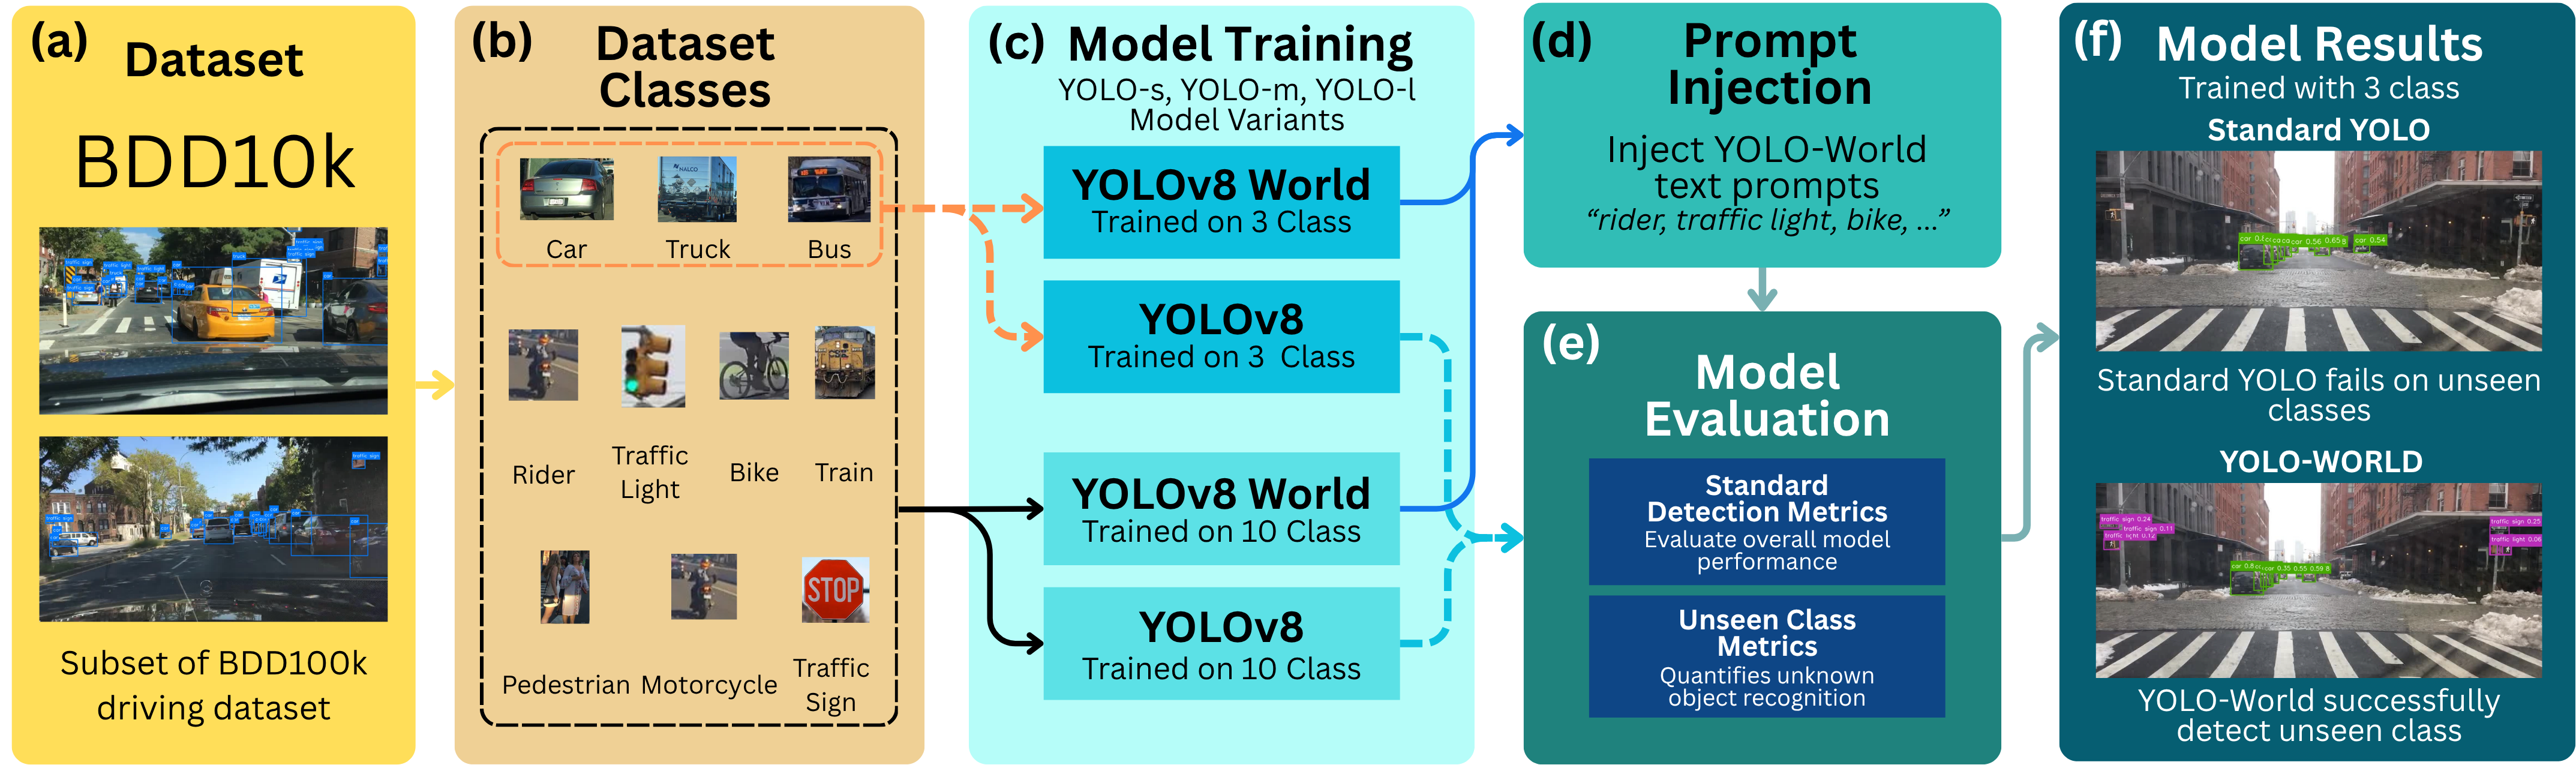
\includegraphics[width=0.96\textwidth]{figs/Flowchart.png}
\caption{Comprehensive experimental pipeline and evaluation methodology. (a) BDD 10K dataset configuration. (b) Class distribution for the 3-class and all-class settings. (c) Four experimental training configurations. (d) Semantic text prompt integration for the YOLO-World model. (e) Model evaluation using standard and unseen class metrics. (f) Detection results demonstrating YOLO-World's ability to recognize unseen data.}
\label{fig:fig_1}
\end{figure*}

The rapid advancement of autonomous driving systems relies heavily on the accuracy and robustness of perception modules, particularly object detection \cite{Jebamikyous2022Autonomous, Pravallika2024Deep}. Historically, industry standards have favored closed-set object detection models, such as the widely adopted You Only Look Once architectures \cite{Redmon2015You, Terven2023A}. These models are trained on large, meticulously annotated datasets to achieve real-time inference and high precision for predefined categories. However, their operational capacity is strictly bounded by the classes explicitly registered during the training phase.

Real-world driving environments are dynamic and continuously expose perception systems to edge cases outside standard training distributions. Large-scale benchmarks such as Cityscapes \cite{Cordts2016Cityscapes}, the India Driving Dataset \cite{Varma2018IDD}, ACDC \cite{Sakaridis2021ACDC}, and BDD100K \cite{Yu2018BDD100K} capture diverse urban layouts, traffic structures, weather conditions, and times of day. However, even with this dataset coverage, traditional closed-set models still fail to detect out-of-distribution objects or force them into known categories when those objects are absent from training \cite{Dhamija2020The, Li2025Out-of-distribution}. In autonomous navigation, this limitation creates safety hazards because planning systems may remain blind to critical obstacles and corner cases \cite{Li2022CODA, Chen2025INSIGHT}.

To mitigate the vulnerabilities of closed-set paradigms, the field is increasingly shifting towards Vision-Language Models and Open-Vocabulary Object Detection frameworks \cite{Radford2021Learning, Li2024From}. By aligning visual features with natural language text embeddings, these open-vocabulary frameworks can recognize arbitrary categories specified via text prompts without requiring domain-specific retraining. Among recent developments, YOLO-World \cite{Cheng2024YOLO-World} emerges as a state-of-the-art solution, combining the real-time efficiency of standard YOLO architectures with open-vocabulary, zero-shot detection capabilities. This enables the model to identify unfamiliar objects on the fly, drastically improving situational awareness.




The primary goal of this research is to comprehensively evaluate the capacity of open-vocabulary object detection systems to mitigate the inherent safety hazards posed by closed-set limitations in autonomous driving. Specifically, the zero-shot detection reliability of the YOLO-World architecture is empirically assessed against standard YOLO models when confronted with unfamiliar or unlearned objects. To conduct this evaluation, a specific data subset derived from the diverse BDD100K driving dataset, referred to as BDD10K, is utilized.utilized.

Throughout this paper, the term \textit{Target Classes} denotes object categories that are explicitly registered, learned, and optimized during the model training or fine-tuning phase. Conversely, \textit{Unknown Classes} refer to out-of-distribution road objects that are deliberately excluded from supervised optimization and encountered strictly during inference. Although these concepts are broadly applicable to open-vocabulary detection, this study defines the Target Classes exclusively as three vehicle categories, namely car, bus, and truck. The Unknown Classes comprise the remaining seven unlearned road-hazard categories: pedestrian, rider, train, motorcycle, bicycle, traffic light, and traffic sign.

To achieve this goal, the study follows the structured pipeline in Fig. \ref{fig:fig_1}. The BDD10K subset is first pre-processed through category alias mapping and label normalization, as shown in Fig. \ref{fig:fig_1}a, before its class distribution is organized into all-class and target-class settings in Fig. \ref{fig:fig_1}b. The models are then trained across Small, Medium, and Large variants under the experimental configurations in Fig.~\ref{fig:fig_1}c, while YOLO-World additionally receives semantic class prompts as illustrated in Fig.~\ref{fig:fig_1}d. Evaluation combines standard and unseen-class metrics, including ${mAP_{50}}$ and class-agnostic misclassification analysis, as summarized in Fig. \ref{fig:fig_1}e, and the resulting detections in Fig. \ref{fig:fig_1}f provide qualitative evidence of open-vocabulary recognition for unseen road objects.

\begin{figure*}[!ht]
\centering
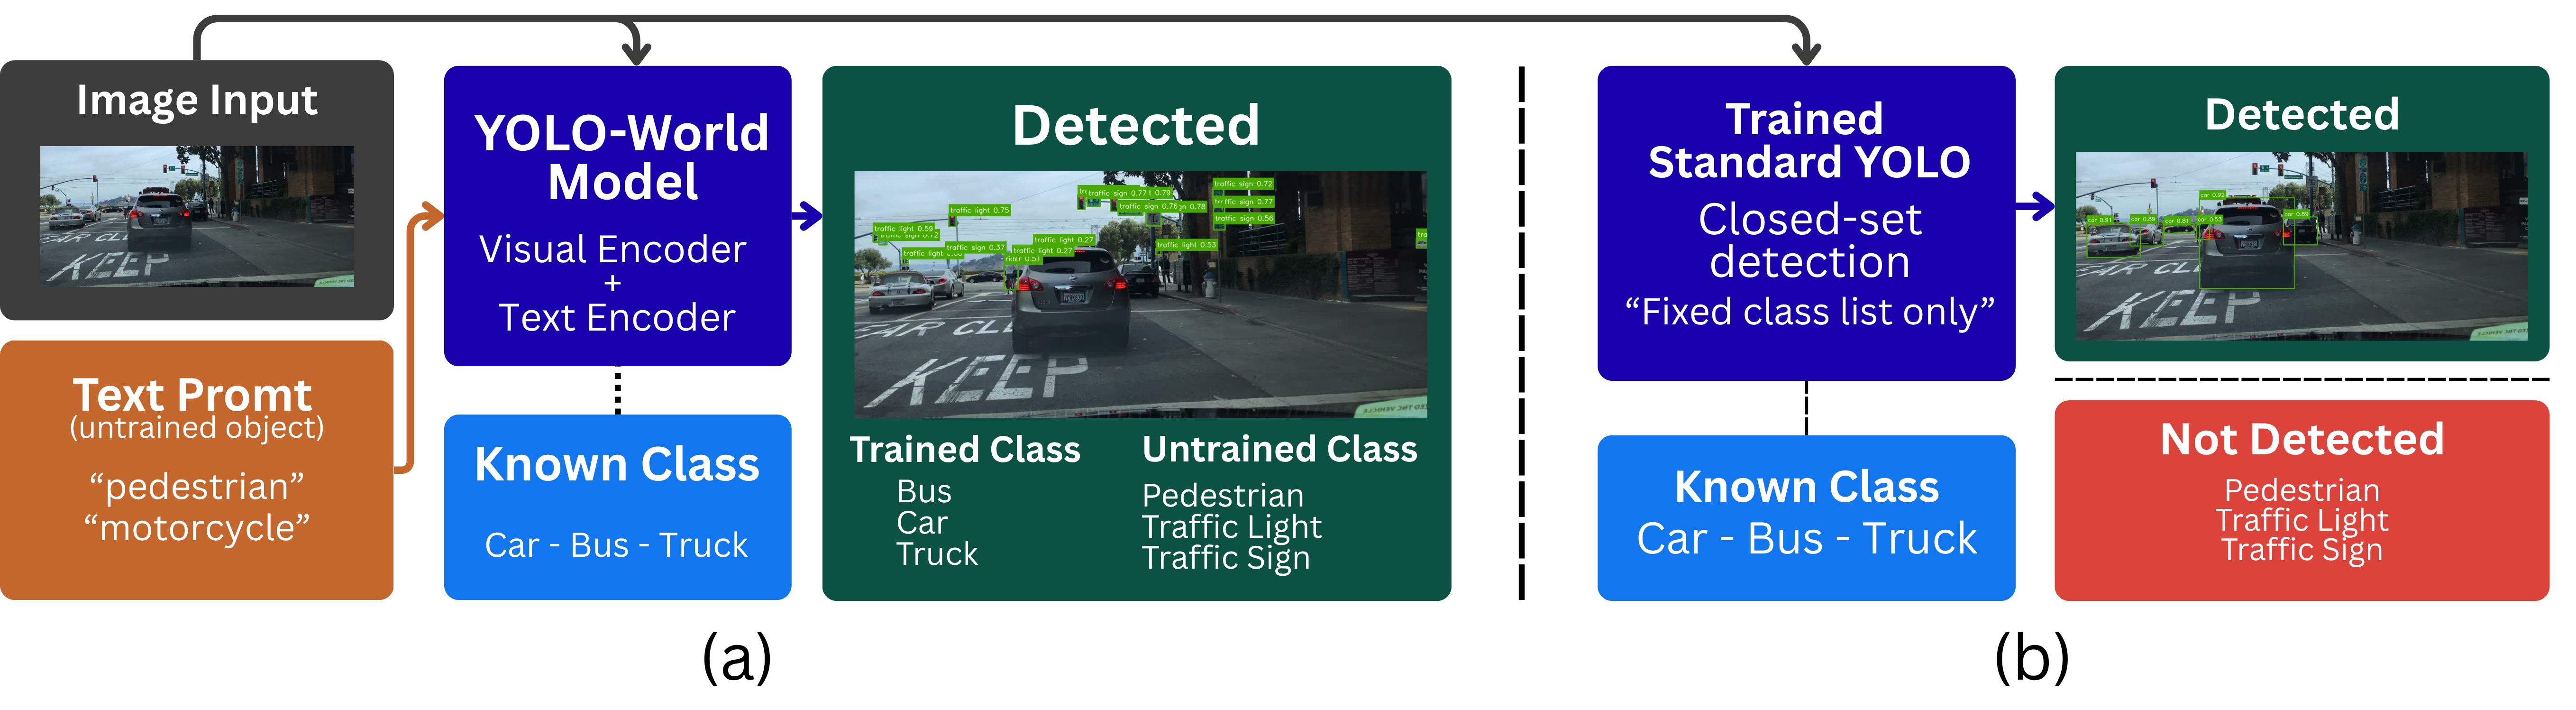
\includegraphics[width=0.96\textwidth]{figs/Flowchart_comparison.png}
\caption{Input-output modality comparison. (a) YOLO-World's dual-modality framework for open-vocabulary detection. (b) Standard YOLO's single-modality framework for closed-set detection.}
\label{fig:fig_2}
\end{figure*}

\section{Related Work}
\label{sec:related_work}

The evolution of real-time object detection has been significantly shaped by the You Only Look Once architectures \cite{Redmon2015You, Terven2023A, Diwan2022Object, Vijayakumar2024YOLO-based}, which traditionally operate under closed-vocabulary assumptions and require predefined categories. Recent open-vocabulary and zero-shot detectors, especially YOLO-World \cite{Cheng2024YOLO-World}, extend this paradigm by combining vision-language models with prompt-based localization \cite{Radford2021Learning, Gu2021Open-vocabulary, Du2022Learning}. This shift enables detection of categories specified through language prompts and responds to dynamic environments where unknown classes frequently appear \cite{Iqbal2024Redefining, Li2024From, Schmarje2024UNCOVER}.

Robust autonomous-driving detection also depends on diverse evaluation data, including BDD100K \cite{Yu2018BDD100K}, Cityscapes \cite{Cordts2016Cityscapes}, IDD \cite{Varma2018IDD}, ACDC \cite{Sakaridis2021ACDC}, and CODA \cite{Li2022CODA}, which expose models to urban variation, adverse conditions, and road corner cases \cite{Liu2024Benchmarking, Chhipa2024Open-Vocabulary}. Efficiency-oriented driving studies report useful closed-set references: Gupta et al. \cite{10605392} obtain BDD10K mAP values of 20.08--23.35\%, Geever et al. \cite{11376542} show that downsampling choices change average precision by less than 2\%, and Li et al. \cite{10550965} improve vehicle detection under difficult lighting and spatial constraints. The BDD100K model zoo further reports 10-class Box AP values of 32.71\%, 33.72\%, and 31.13\% for Faster R-CNN R-101-FPN, Cascade R-CNN R-50-FPN, and FCOS R-101-FPN, respectively \cite{bdd100kModelZoo}; however, these references still primarily reflect known-class detection.

Zero-shot and prompt-guided models have also been adapted beyond autonomous driving. Mullins et al. \cite{agronomy14122830} evaluated YOLO-World and Grounding DINO for wild blueberry annotation, where Grounding DINO achieved 0.642 mIoU compared with 0.503 mIoU for YOLO-World. In manufacturing, Tang et al. \cite{Tang2025Prompt} applied prompt-guided AI analytics to digital twins, showing that vision-language detection can transfer to specialized industrial objects. These studies demonstrate broad flexibility, but their domain shift, computational overhead, and imperfect zero-shot precision leave open questions for safety-critical road scenes.

Despite these advances, open-vocabulary detection has not been sufficiently validated against established closed-set standards for unseen autonomous-driving hazards. Existing literature largely reports known-class detection accuracy, domain-transfer results, or efficiency trade-offs, while the safety-critical question of whether a detector can recover road objects excluded from training remains unresolved. Therefore, this research directly compares YOLO-World with Standard YOLOv8 on BDD10K, focusing on unseen classes under controlled open-vocabulary and closed-set evaluation protocols.


\section{Research Methodology}
\subsection{Research Architecture}


The comparative models differ primarily in input modality and classification paradigm, as conceptualized in Fig. \ref{fig:fig_2}. Standard YOLOv8, shown in Fig. \ref{fig:fig_2}b, follows a closed-set single-modality design that maps visual features to fixed classification heads learned during training; therefore, out-of-distribution objects are either ignored as background or forced into known labels. YOLO-World, shown in Fig. \ref{fig:fig_2}a, uses an open-vocabulary dual-modality design that conditions visual detection on semantic text prompts, enabling novel object localization without structural retraining.

To evaluate this disparity in autonomous driving, the study uses the BDD10K multi-scheme pipeline in Fig. \ref{fig:fig_1} across Small (s), Medium (m), and Large (l) variants. The all-class track trains both architectures on the full 10-class set to establish a supervised upper bound, while the Target-Class track trains only on three vehicle classes and withholds seven Unknown Classes. In the latter setting, YOLO-World is queried for unseen categories through text prompts, whereas Standard YOLOv8 is analyzed through class-agnostic recall, forced misclassification, and miss-rate behavior, isolating open-vocabulary adaptability from closed-set failure modes.

\subsection{Dataset Configuration}
This research utilizes BDD10K, a curated and label-normalized subset derived from the larger BDD100K driving dataset. Model optimization uses images and annotations from the standard \texttt{train} folder, while validation, zero-shot testing, and metric computation are performed strictly on the \texttt{val} split. The official BDD100K \texttt{test} split is excluded because its ground-truth labels are withheld, preventing exact bounding-box evaluation for $mAP_{50}$, $mAP_{50-95}$, precision, recall, and F1-score. The ten mapped categories are car, bus, truck, pedestrian, rider, train, motorcycle, bicycle, traffic light, and traffic sign.

Within this study, the categories are partitioned into three Target Classes, namely car, bus, and truck, and seven Unknown Classes, namely pedestrian, rider, train, motorcycle, bicycle, traffic light, and traffic sign. As shown in Table~\ref{tab:bdd10k_class_distribution}, Target Classes account for approximately 64.5\% of training instances and 64.0\% of combined train-validation instances, while Unknown Classes account for 35.5\% and 36.0\%, respectively. This deliberately imbalanced 3:7 split emulates a safety-critical setting in which dominant vehicle classes are supervised while vulnerable road users, traffic-control devices, and rarer hazards must still be detected. The shared \texttt{val} split preserves ground truth for both groups, ensuring that Unknown Class detections by YOLO-World reflect prompt-conditioned transfer rather than direct exposure during Target-Class fine-tuning.

\begin{table}[htbp]
\caption{BDD10K Class Distribution across Training and Validation Splits}
\begin{center}
\begin{tabular}{|l|l|l|l|}
\hline
\textbf{Category Name} & \textbf{Train Instances} & \textbf{Val Instances} & \textbf{Total Instances} \\
\hline
car & 72000 (60.0\%) & 5141 (54.4\%) & 77141 (59.6\%) \\
bus & 1800 (1.5\%) & 88 (0.9\%) & 1888 (1.5\%) \\
truck & 3600 (3.0\%) & 246 (2.6\%) & 3846 (3.0\%) \\
pedestrian & 21600 (18.0\%) & 871 (9.2\%) & 22471 (17.4\%) \\
rider & 1800 (1.5\%) & 39 (0.4\%) & 1839 (1.4\%) \\
train & 240 (0.2\%) & 0 (0.0\%) & 240 (0.2\%) \\
motorcycle & 1200 (1.0\%) & 20 (0.2\%) & 1220 (0.9\%) \\
bicycle & 3600 (3.0\%) & 67 (0.7\%) & 3667 (2.8\%) \\
traffic light & 7200 (6.0\%) & 1191 (12.6\%) & 8391 (6.5\%) \\
traffic sign & 6960 (5.8\%) & 1763 (18.7\%) & 8723 (6.7\%) \\
\hline
\end{tabular}
\label{tab:bdd10k_class_distribution}
\end{center}
% TODO: Author to replace with exact script counts
\end{table}

\subsection{YOLO \& YOLO-World Model}
Both detection paradigms are tested using Small (s), Medium (m), and Large (l) scales to assess whether open-vocabulary awareness remains feasible across lightweight, mid-range, and high-capacity inference budgets. The shared optimization settings are listed in Table~\ref{tab:training_hyperparameters}, and parameter/GFLOPs complexity is summarized in Table~\ref{tab:model_complexity_runner_logs}. Architecturally, Standard YOLOv8 is treated as a single-modality closed-set baseline whose fixed classification head cannot emit categories absent from supervised training, as illustrated in Fig.~\ref{fig:fig_architecture_yolov8}; YOLO-World is treated as a dual-modality detector that injects natural-language prompts through CLIP-based text embeddings to support zero-shot recognition, as illustrated in Fig.~\ref{fig:fig_architecture_yolo_world} \cite{paperyolo-world}.


\begin{figure}
    \centering
    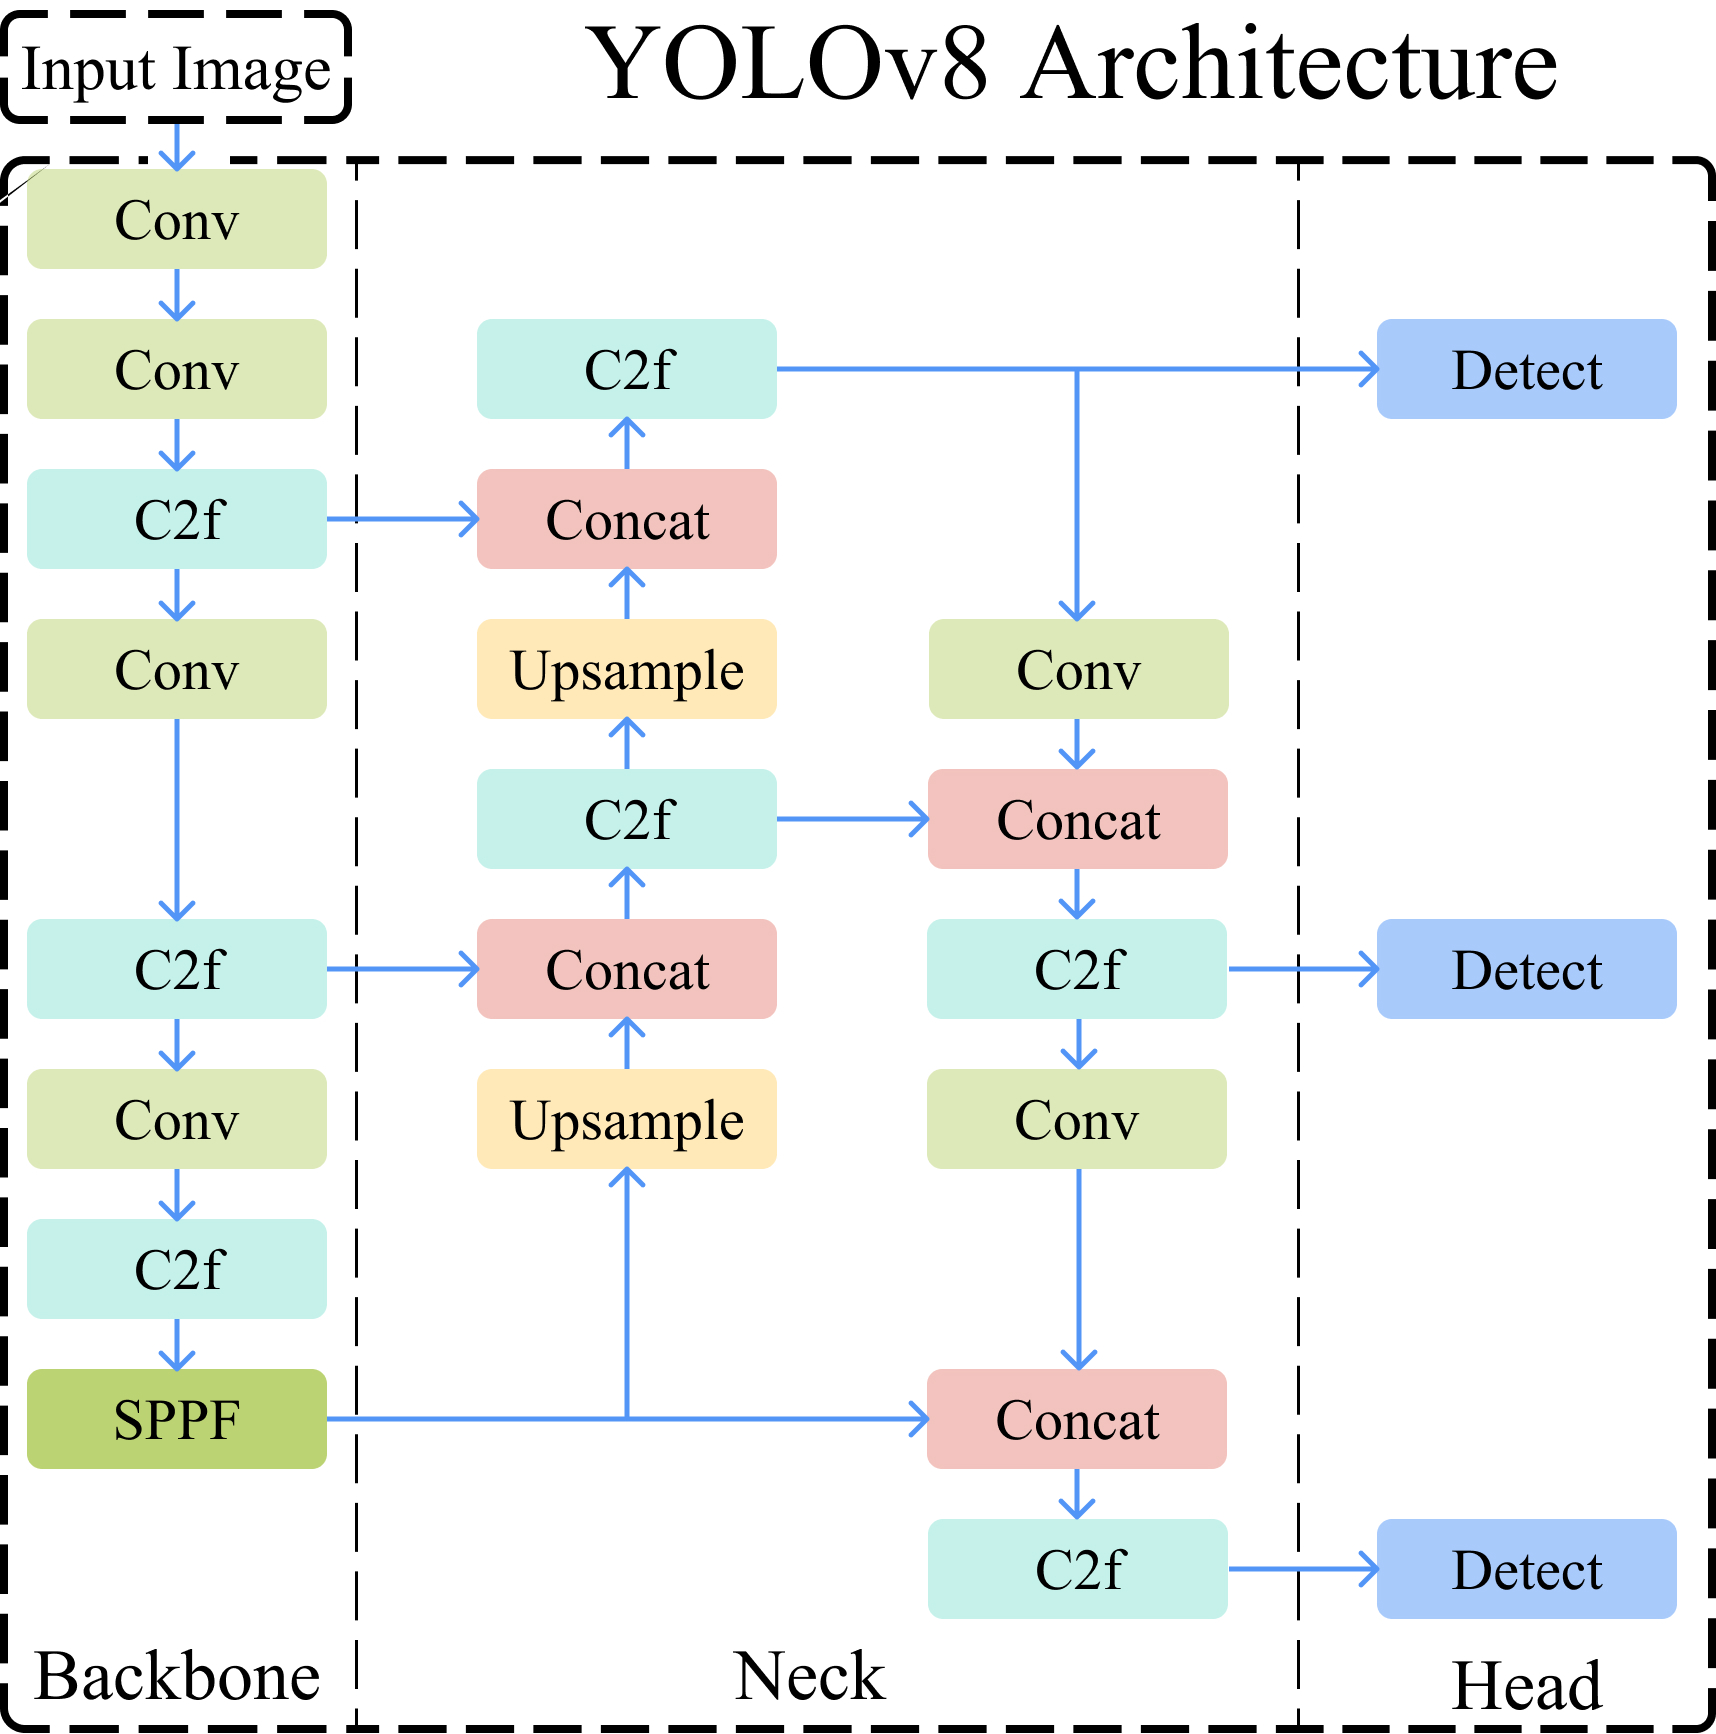
\includegraphics[width=0.75\columnwidth]{figs/yolov8.jpeg}
    \caption{YOLOv8 Architecture Overview.}
    \label{fig:fig_architecture_yolov8}
\end{figure}


\begin{figure}
    \centering
    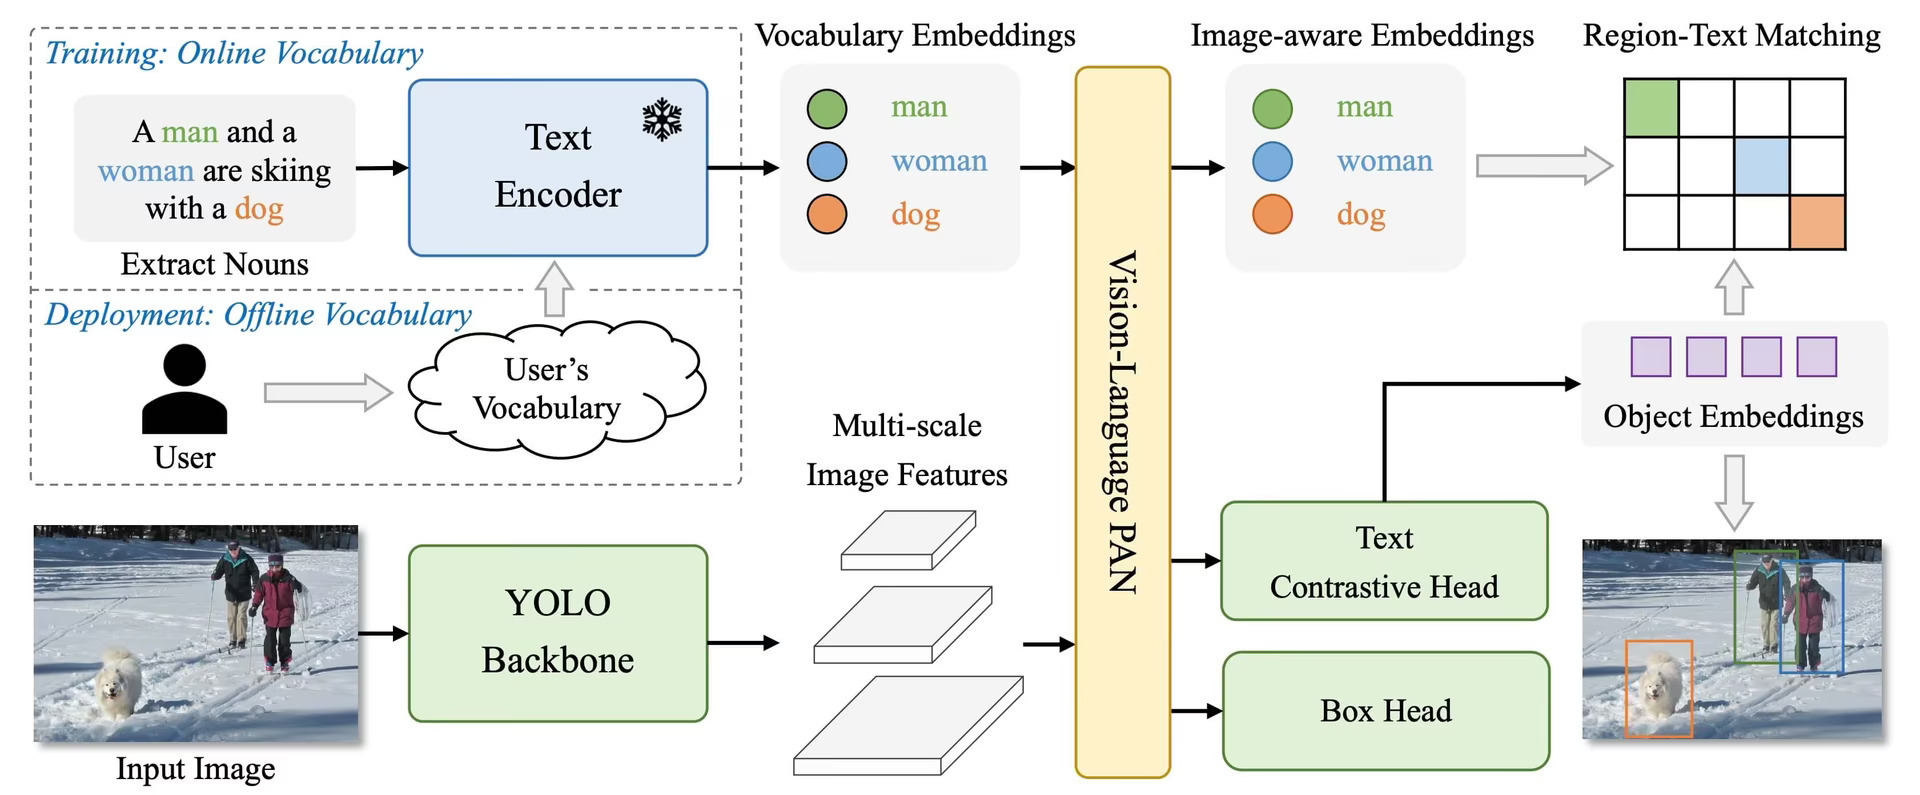
\includegraphics[width=0.96\columnwidth]{figs/yolo-world.jpg}
    \caption{YOLO-World Architecture Overview. \cite{paperyolo-world}}
    \label{fig:fig_architecture_yolo_world}
\end{figure}




\begin{table}[htbp]
\caption{Default Hyperparameter Configurations for Model Optimization}
\begin{center}
\begin{tabular}{|l|c|}
\hline
\textbf{Hyperparameter} & \textbf{Value} \\
\hline
Optimizer & AdamW \\
Epochs & 50 \\
Initial learning rate & 0.001 \\
Momentum & 0.937 \\
Weight decay & 0.0005 \\
NMS IoU threshold & 0.7 \\
Confidence threshold & 0.001 \\
\hline
\end{tabular}
\label{tab:training_hyperparameters}
\end{center}
\end{table}

\begin{table}[htbp]
\caption{Model Parameters and GFLOPs Used in Training}
\begin{center}
\begin{tabular}{|l|c|c|c|}
\hline
\textbf{Model} & \textbf{Scale} & \textbf{Params (M)} & \textbf{GFLOPs} \\
\hline
YOLO-World & Small & 13.3835 & 40.1 \\
YOLO-World & Medium & 29.0653 & 94.5 \\
YOLO-World & Large & 47.5540 & 185.1 \\
\hline
YOLOv8 & Small & 11.1395 & 28.7 \\
YOLOv8 YOLO & Medium & 25.8621 & 79.1 \\
YOLOv8 YOLO & Large & 43.6376 & 165.4 \\
\hline
\end{tabular}
\label{tab:model_complexity_runner_logs}
\end{center}
\end{table}




The complexity comparison in Table~\ref{tab:model_complexity_runner_logs} shows that YOLO-World consistently requires more parameters and GFLOPs than Standard YOLOv8 at the same scale, reflecting the overhead of vision-language alignment and prompt-conditioned detection. This cost is evaluated against the safety benefit of open-vocabulary awareness in autonomous-driving perception. In addition to the fine-tuned configurations, the study includes a pure pretrained YOLO-World baseline in which the ten BDD10K class prompts are injected into a frozen off-the-shelf checkpoint, establishing a no-fine-tuning reference for pretrained semantic alignment.


\subsection{Training Methodology}
Five experimental schemes are applied across the Small, Medium, and Large variants, yielding fifteen model runs in total. Scheme 1 is the pure pretrained YOLO-World baseline, in which zero classes are trained and all ten BDD10K categories are queried through zero-shot text prompts. Scheme 2 is YOLO-World All-Class, where the model is fine-tuned on all ten mapped categories through prompt-guided supervision. Scheme 3 is YOLO-World Target-Class, where fine-tuning is restricted to the three Target Classes through prompts while the seven Unknown Classes remain excluded from supervised optimization. Scheme 4 is Standard YOLO All-Class, where the detector is fine-tuned on all ten categories using a ten-class closed-set head. Scheme 5 is Standard YOLO Target-Class, where the detector is fine-tuned only on car, bus, and truck using a three-class closed-set head.

The key control mechanism in Scheme 3 and Scheme 5 is the removal of Unknown Class supervision during training. If a training image contains a car as a Target Class and a pedestrian as an Unknown Class, the pedestrian bounding box is stripped from the training label file and contributes no positive detection target. In practical terms, the Unknown Class region is absorbed into the background loss rather than being optimized as a semantic object category. This masking protocol guarantees that the fine-tuned visual weights receive no direct category-level supervision for the seven Unknown Classes, thereby making subsequent detection of those classes a genuine test of open-vocabulary generalization rather than supervised memorization.

\subsection{Evaluation Methodology}
Evaluation is performed on the BDD10K \texttt{val} split in two stages. The first stage measures detection performance across all ten categories, where YOLO-World parses the full prompt array, namely ``car'', ``bus'', ``truck'', ``pedestrian'', ``rider'', ``train'', ``motorcycle'', ``bicycle'', ``traffic light'', and ``traffic sign'', while Standard YOLOv8 uses its fixed closed-set classification head. For Scheme 5, the three-class Standard YOLOv8 model has no output channels for the seven Unknown Classes, so missed unknown objects are treated as 100\% false negatives wherever corresponding ground-truth boxes exist, lowering aggregate $mAP_{50}$, $mAP_{50-95}$, recall, and F1-score. The second stage isolates the Unknown Classes to test whether Scheme 3, YOLO-World fine-tuned only on vehicle Target Classes, can still detect unseen road hazards through text prompts without supervised examples of those categories.

Failure analysis under the Target-Class setting combines class-agnostic and class-specific measurements. Class-Agnostic Recall measures whether an Unknown Class object is localized regardless of its predicted label, Miss Rate quantifies ground-truth Unknown Class objects with no valid detection, and forced misclassification records cases where unknown objects are projected onto known vehicle labels, revealing the safety limitation of static closed-set classifiers. Because autonomous-driving perception also requires real-time feasibility, each model scale is benchmarked using parameter count and inference latency, allowing the study to compare semantic flexibility, detection accuracy, and deployment cost across Small, Medium, and Large variants.

\section{Results and Discussion}

\subsection{Experiment Result}

\begin{table*}[htbp]
\caption{Comprehensive Detection Performance across Scaling Variants with Gain over YOLO-World Zero-Shot Baseline ($mAP_{50}$)}
\begin{center}
\footnotesize
\begin{tabular*}{\textwidth}{@{\extracolsep{\fill}}lcccc@{}}
\hline
\textbf{Experimental Scheme} & \textbf{Evaluation Target} & \textbf{Small} & \textbf{Medium} & \textbf{Large} \\
\hline
YOLO-World Zero-Shot Baseline & \multirow{5}{*}{\begin{tabular}{c}All-Class\\Evaluation\end{tabular}} & 18.27\% (Ref.) & 20.57\% (Ref.) & 21.45\% (Ref.) \\
YOLOv8 3-Class Trained &  & 15.94\% (-2.33) & 16.56\% (-4.01) & 16.76\% (-4.69) \\
YOLOv8 10-Class Trained &  & 28.55\% (+10.28) & 31.17\% (+10.60) & 31.77\% (+10.32) \\
YOLO-World 3-Class Trained &  & 28.02\% (+9.75) & 30.59\% (+10.02) & 30.35\% (+8.90) \\
YOLO-World 10-Class Trained &  & 27.63\% (+9.36) & 30.82\% (+10.25) & 33.50\% (+12.05) \\
\hline
YOLO-World Zero-Shot Baseline & \multirow{5}{*}{\begin{tabular}{c}Unknown-Class\\Evaluation\end{tabular}} & 12.36\% (Ref.) & 13.52\% (Ref.) & 14.79\% (Ref.) \\
YOLOv8 3-Class Trained &  & 0.00\% (-12.36) & 0.00\% (-13.52) & 0.00\% (-14.79) \\
YOLOv8 10-Class Trained &  & 19.07\% (+6.71) & 21.14\% (+7.62) & 21.43\% (+6.64) \\
YOLO-World 3-Class Trained &  & 19.67\% (+7.31) & 19.67\% (+6.15) & 19.67\% (+4.88) \\
YOLO-World 10-Class Trained &  & 16.89\% (+4.53) & 21.43\% (+7.91) & 23.73\% (+8.94) \\
\hline
\end{tabular*}
\normalsize
\label{tab:comprehensive_map50_results}
\end{center}
\end{table*}

\begin{figure}
    \centering
    \includegraphics[width=0.96\columnwidth]{figs/Yolo_Comparison_Result.png}
    \caption{Fig. 5. Prediction omparison on a BDD10K test dataset. (a) Ground-truth (b) Baseline YOLO-World Large (c) YOLOv8l - 3 Classes (d) YOLO-World large - 3 Classes. (e) YOLOv8l - 10 Classes (f) YOLO-World Large - 10 Classes}
    \label{fig:fig_yolo_result_comparison}
\end{figure}

Table~\ref{tab:comprehensive_map50_results} reports the $mAP_{50}$ performance across the Small, Medium, and Large scaling variants. In the fully supervised 10-class setting, YOLO-World reaches 33.50\% $mAP_{50}$ at the Large scale, exceeding the corresponding Standard YOLOv8 result of 31.77\% by approximately 1.72 percentage points. This margin is important because both models receive full category supervision under this setting; therefore, the advantage cannot be attributed merely to access to additional labels. Instead, it indicates that cross-modal visual-semantic alignment can produce richer discriminative representations than a purely visual closed-set backbone, particularly when model capacity increases. Although the Small and Medium variants remain closely matched, the Large-scale supervised ceiling suggests that the semantic conditioning mechanism in YOLO-World becomes increasingly beneficial as representational capacity grows.

The most significant result is observed in the open-vocabulary evaluation. The pure pretrained YOLO-World baseline achieves non-zero unknown-class $mAP_{50}$ across all scales, confirming that pretrained vision-language alignment already provides limited zero-shot transfer to BDD10K road objects. However, after fine-tuning YOLO-World on only the three Target Classes, the unknown-class score rises to 19.67\% $mAP_{50}$, corresponding to the reported +6.64\% improvement over the pure zero-shot baseline. This empirical behavior suggests that target-domain fine-tuning on vehicles improves the localization anchors, road-scene priors, and feature calibration of the detector without erasing its semantic ability to respond to unseen prompt categories. In strict contrast, Standard YOLOv8 trained on the same three Target Classes obtains a mathematical 0.00\% $mAP_{50}$ on Unknown Classes because its closed-set detection head has no output channel for pedestrian, rider, train, motorcycle, bicycle, traffic light, or traffic sign.

Fig.~\ref{fig:fig_yolo_result_comparison} provides a qualitative dissection of the same phenomenon under a dense urban-intersection scene. Sub-figure (a) contains 28 ground-truth objects distributed across vehicles, pedestrians, traffic lights, and traffic signs. The pretrained YOLO-World baseline in sub-figure (b) detects 13 objects, demonstrating useful but incomplete semantic transfer, with visible difficulty on small or occluded traffic signs. The safety failure is most apparent in sub-figure (c), where Standard YOLOv8 trained only on three Target Classes detects exactly 6 vehicle objects while remaining blind to traffic lights, signs, and pedestrians. In an autonomous-driving context, this is a silent hazard: the perception module produces no warning for unlearned vulnerable road users or traffic-control objects. By contrast, sub-figure (d) shows YOLO-World trained on the same three Target Classes detecting 32 objects, including target vehicles and unlearned pedestrians and traffic lights through text prompts. The difference between 32 detections and 28 ground-truth objects should not be interpreted solely as superior recall; it also reflects a granular over-splitting tendency of prompt-guided contrastive heads on distant contextual objects, where semantically similar or partially occluded regions may be localized as multiple candidate instances.

\subsection{Discussion}

\begin{table*}[htbp]
\caption{Metric Comparison with Related Object Detection Studies}
\begin{center}
\begin{tabular*}{\textwidth}{@{\extracolsep{\fill}}lllcccc}
\hline
\textbf{Model / Study} & \textbf{Dataset} & \textbf{Evaluation Set} & \textbf{$mAP_{50}$} & \textbf{$mAP_{50-95}$} & \textbf{mAP} & \textbf{mIoU} \\
\hline
Energy-adaptive NAS \cite{10605392} & BDD10K & 10 Class & -- & -- & 20.08--23.35\% & -- \\
Downsampling analysis \cite{11376542} & BDD10K & 10 Class & -- & -- & $\Delta$AP $<2\%$ & -- \\
Faster R-CNN R-101-FPN \cite{bdd100kModelZoo} & BDD100K & 10 Class & 32.71\% & -- & -- & -- \\
Cascade R-CNN R-50-FPN \cite{bdd100kModelZoo} & BDD100K & 10 Class & 33.72\% & -- & -- & -- \\
FCOS R-101-FPN \cite{bdd100kModelZoo} & BDD100K & 10 Class & 31.13\% & -- & -- & -- \\
YOLO-World \cite{agronomy14122830} & Agriculture & Object Localization & -- & -- & -- & 0.503 \\
Grounding DINO \cite{agronomy14122830} & Agriculture & Object Localization & -- & -- & -- & 0.642 \\
\textbf{YOLOv8-L 3-Class} & BDD10K & 10 Class & 16.76\% & 11.68\% & 11.68\% & 0.2164 \\
\textbf{YOLOv8-L 10-Class} & BDD10K & 10 Class & 31.77\% & 19.32\% & 19.32\% & 0.6628 \\
\textbf{YOLO-World-L Zero-Shot} & BDD10K & 10 Class & 21.45\% & 14.90\% & 14.90\% & 0.6220 \\
\textbf{YOLO-World-L 3-Class} & BDD10K & 10 Class & 30.35\% & 18.37\% & 18.37\% & 0.7040 \\
\textbf{YOLO-World-L 10-Class} & BDD10K & 10 Class & 33.50\% & 19.66\% & 19.66\% & 0.6752 \\
\hline
\end{tabular*}
\label{tab:related_work_comparison}
\end{center}
\end{table*}

The comparison in Table~\ref{tab:related_work_comparison} positions the proposed experiments relative to prior object-detection studies already discussed in the related work. Gupta et al. \cite{10605392} report BDD10K mAP values between 20.08\% and 23.35\% for energy-efficient closed-set ADAS detectors, which is relevant as an edge-deployment reference but does not address semantic recovery of unseen categories. Geever et al. \cite{11376542} primarily analyze image downsampling and interpolation effects, reporting an average-precision variation below 2\%, which confirms that preprocessing can affect efficiency while leaving the closed-set label assumption unchanged. The BDD100K model zoo further reports 10-class Box AP values of 32.71\%, 33.72\%, and 31.13\% for Faster R-CNN R-101-FPN, Cascade R-CNN R-50-FPN, and FCOS R-101-FPN, respectively \cite{bdd100kModelZoo}. These values provide a closer road-scene reference than non-driving datasets, although they are still not fully identical to the curated BDD10K subset and protocol used in this study. Mullins et al. \cite{agronomy14122830} demonstrate the transferability of YOLO-World in an agricultural zero-shot scenario, where YOLO-World and Grounding DINO obtain mIoU values of 0.503 and 0.642, respectively. These agricultural values are not directly comparable to road-scene $mAP_{50}$ because they use a different dataset, domain, and evaluation protocol, but they provide useful context for evaluating prompt-guided object localization. Under the BDD10K validation protocol used in this study, the Large-scale comparison shows that YOLO-World-L improves from 21.45\% $mAP_{50}$ in the zero-shot setting to 30.35\% after three-class target fine-tuning and 33.50\% after full ten-class fine-tuning. The corresponding YOLOv8-L 3-class and 10-class results of 16.76\% and 31.77\% indicate that prompt-conditioned vision-language representations provide stronger cross-category transfer while still remaining competitive under fully supervised evaluation.

These quantitative and qualitative results translate directly into autonomous-driving safety implications. A downstream planner does not consume $mAP_{50}$ as an abstract number; it consumes object hypotheses that define whether the vehicle should continue, yield, brake, or replan. Therefore, reducing Class-Agnostic Miss Rates is not merely an accuracy improvement but a prerequisite for robust robotic decision-making. A closed-set detector that assigns 0.00\% unknown-class $mAP_{50}$ can silently remove pedestrians, traffic lights, or riders from the world model, leaving path-planning and emergency-braking modules with incomplete scene state. Open-vocabulary prompting mitigates this failure mode by allowing the perception system to query safety-critical concepts beyond the supervised label set. For autonomous navigation in dynamic environments, this capacity is non-negotiable because the cost of an unclassified object is not only a lower benchmark score, but a potentially unsafe control decision.

\section{Conclusion}

This paper presents Open-Vocabulary Hazard Perception for Autonomous Driving, a comparative study of Standard YOLOv8 and YOLO-World on the BDD10K road-scene dataset under closed-set and open-vocabulary evaluation protocols. In the fully supervised 10-class setting, YOLO-World-L achieves 33.50\% $mAP_{50}$ compared with 31.77\% for YOLOv8-L, while in the Target-Class setting YOLO-World remains responsive to unlearned road objects and Standard YOLOv8 with a three-class head obtains 0.00\% $mAP_{50}$ on Unknown Classes because its closed-set classifier cannot emit labels excluded from training. These findings show that detectors optimized only for known categories can silently ignore unregistered hazards, whereas text-conditioned YOLO-World can query safety-critical objects beyond the supervised label set. The study contributes a controlled BDD10K Target/Unknown evaluation protocol, a scale-wise comparison across Small, Medium, and Large variants, and a combined quantitative and qualitative analysis of closed-set failure versus prompt-conditioned road-object awareness. Future work should extend the evaluation to larger validation splits, adverse weather and nighttime conditions, temporal video detection, downstream planning simulation, prompt engineering, uncertainty calibration, and real-time deployment constraints.


\bibliographystyle{IEEEtran}

\bibliography{references}
\end{document}
